\chapter{Introduction}
\section{Repository Links}
\begin{itemize}
    \item Dissertation (Repository): \ur{https://github.com/johnshields/Repota-Database} % Database Repository
    \item Repota (Repository): \url{https://github.com/johnshields/AP-MD-FYP} % Application Repository
    \item Horton (Repository): \ur{https://github.com/johnshields/Horton} % Back-end Server Repository
    \item Database (Repository): \ur{https://github.com/johnshields/Repota-Database} % Database Repository

\end{itemize}
\section{Project Introduction}
The purpose of this project was to construct a service report application. Many if not all technicians for car and machinery rental companies have to do a report of a repair or service that is carried out on a vehicle. This is usually handwritten, filled out on Excel or a PDF editor which can be quite tedious.This app will go through a report on a step by step format. There currently is no app for just doing this so I believe this could be a very useful app.
\begin{figure}[h!]
    \caption{Application Icon} % temporary logo
    \label{image:repotaChatLogo}
    \centering
    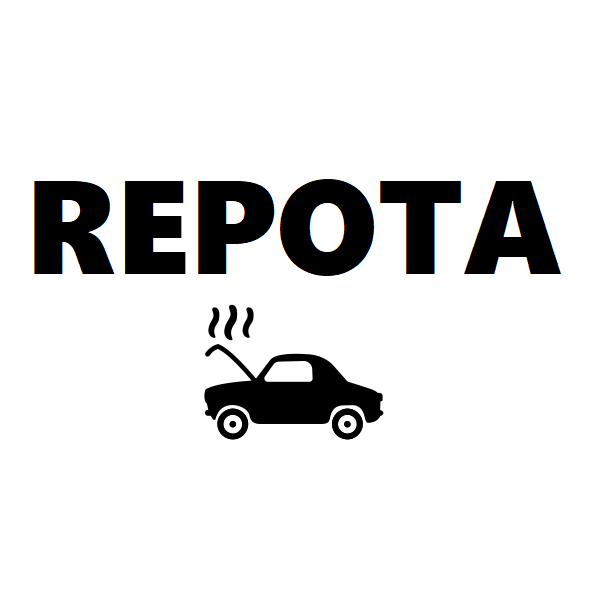
\includegraphics[width=0.8\textwidth]{images/repotaLogo.png}
\end{figure}